% Created 2022-09-23 Fri 10:18
% Intended LaTeX compiler: pdflatex
\documentclass[presentation,aspectratio=169, usenames, dvipsnames]{beamer}
\usepackage[utf8]{inputenc}
\usepackage[T1]{fontenc}
\usepackage{graphicx}
\usepackage{grffile}
\usepackage{longtable}
\usepackage{wrapfig}
\usepackage{rotating}
\usepackage[normalem]{ulem}
\usepackage{amsmath}
\usepackage{textcomp}
\usepackage{amssymb}
\usepackage{capt-of}
\usepackage{hyperref}
\usepackage{khpreamble}
\usepackage{amssymb}
\usepgfplotslibrary{groupplots}
\newcommand*{\shift}{\operatorname{q}}
\definecolor{ppc}{rgb}{0.1,0.1,0.6}
\definecolor{iic}{rgb}{0.6,0.1,0.1}
\definecolor{ddc}{rgb}{0.1,0.6,0.1}
\usetheme{default}
\author{Kjartan Halvorsen}
\date{\today}
\title{Design of control systems}
\hypersetup{
 pdfauthor={Kjartan Halvorsen},
 pdftitle={Design of control systems},
 pdfkeywords={},
 pdfsubject={},
 pdfcreator={Emacs 26.3 (Org mode 9.4.6)}, 
 pdflang={English}}
\begin{document}

\maketitle

\section{Course content}
\label{sec:org6596ac3}

\begin{frame}[label={sec:org9a13a82}]{Feedback control}
\begin{center}
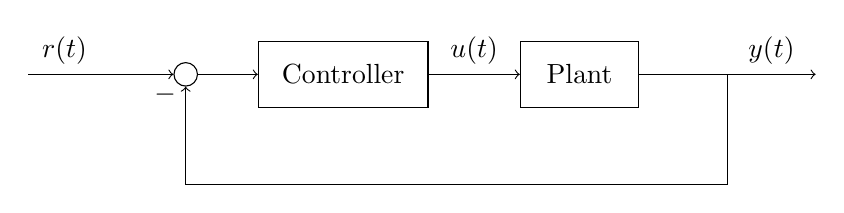
\begin{tikzpicture}[node distance=20mm,
                    block/.style={rectangle, draw, minimum width=15mm, inner sep=3mm},
                    sumnode/.style={circle, draw, inner sep=3pt}]
  \node[coordinate] (input) {};
  \node[sumnode, right of=input] (sum) {};
   \node[block, right of=sum,] (lti) {Controller};
   \node[block, right of=lti, node distance=30mm] (lti2) {Plant};
   \node[coordinate, right of=lti2, node distance=30mm] (output) {};
   \draw[->] (input) -- node[near start, above] {$r(t)$}  (sum);
   \draw[->] (sum) -- node[ above] {}  (lti);
   \draw[->] (lti) -- node[ above] {$u(t)$}  (lti2);
   \draw[->] (lti2) -- node[coordinate] (meas) {} node[near end, above] {$y(t)$} (output);
   \draw[->] (meas) -- ++(0, -14mm) -| node[left, pos=0.96] {$-$} (sum);
 \end{tikzpicture}
\end{center}
\end{frame}


\begin{frame}[label={sec:org9050528}]{Feedback control systems are ubiquitous}
\begin{center}
  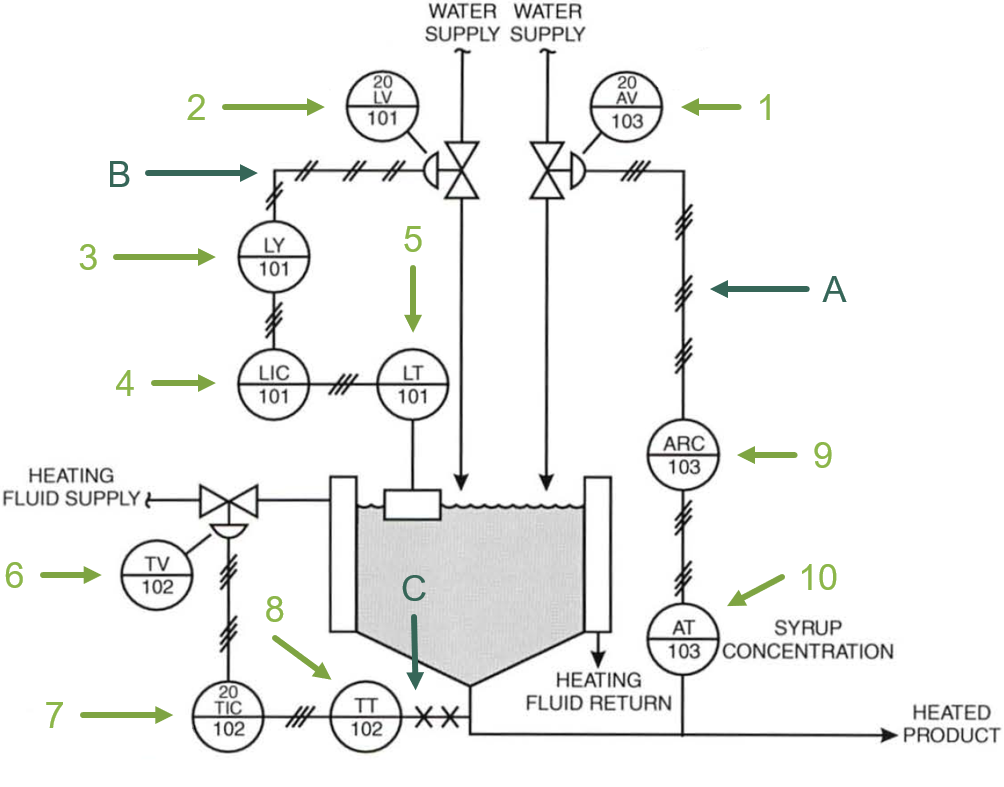
\includegraphics[width=.6\linewidth]{../../figures/PnID-ex.png}
\end{center}
\end{frame}


\begin{frame}[label={sec:orgfe681ff}]{Feedback control systems}
\begin{center}
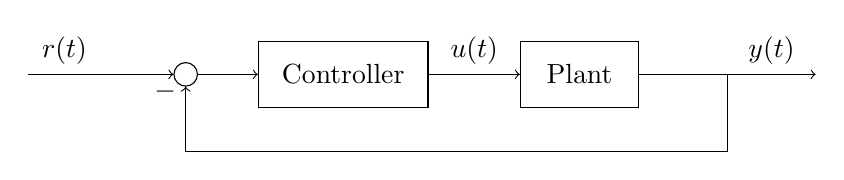
\begin{tikzpicture}[scale = 0.7, node distance=20mm,
                    block/.style={rectangle, draw, minimum width=15mm, inner sep=3mm},
                    sumnode/.style={circle, draw, inner sep=3pt}]
  \node[coordinate] (input) {};
  \node[sumnode, right of=input] (sum) {};
   \node[block, right of=sum,] (lti) {Controller};
   \node[block, right of=lti, node distance=30mm] (lti2) {Plant};
   \node[coordinate, right of=lti2, node distance=30mm] (output) {};
   \draw[->] (input) -- node[near start, above] {$r(t)$}  (sum);
   \draw[->] (sum) -- node[ above] {}  (lti);
   \draw[->] (lti) -- node[ above] {$u(t)$}  (lti2);
   \draw[->] (lti2) -- node[coordinate] (meas) {} node[near end, above] {$y(t)$} (output);
   \draw[->] (meas) -- ++(0, -14mm) -| node[left, pos=0.96] {$-$} (sum);
 \end{tikzpicture}
\end{center}

\alert{Controller design:} Determine a feedback controller such that the controlled system performs according to given \alert{performance specifications}. 
\end{frame}


\begin{frame}[label={sec:orga9b24dc}]{The problem situation}
\begin{columns}
\begin{column}{0.4\columnwidth}
\begin{center}
  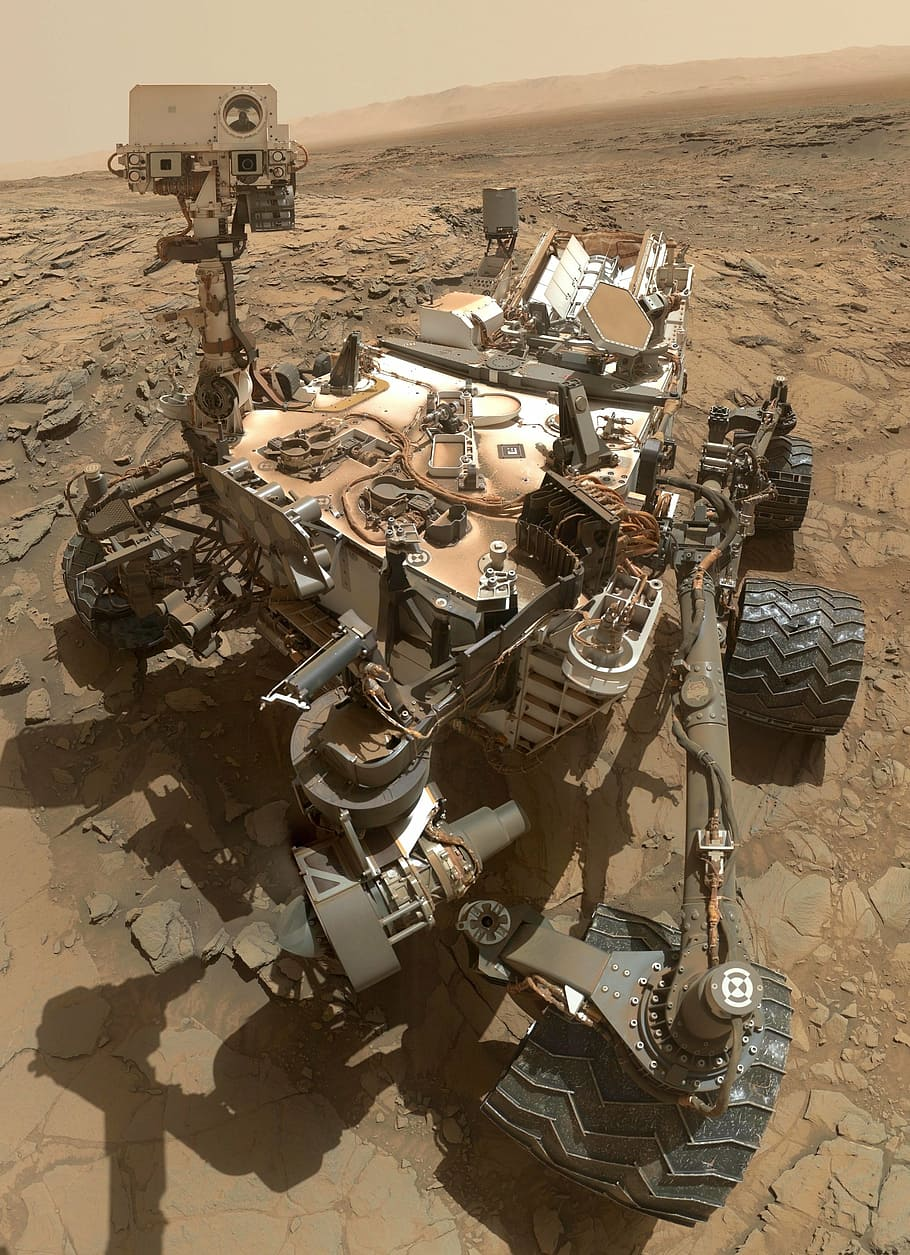
\includegraphics[width=.94\linewidth]{../../figures/mars-rover-curiosity-vehicle-cosmos.jpg}
\end{center}
\end{column}

\begin{column}{0.6\columnwidth}
\begin{center}
  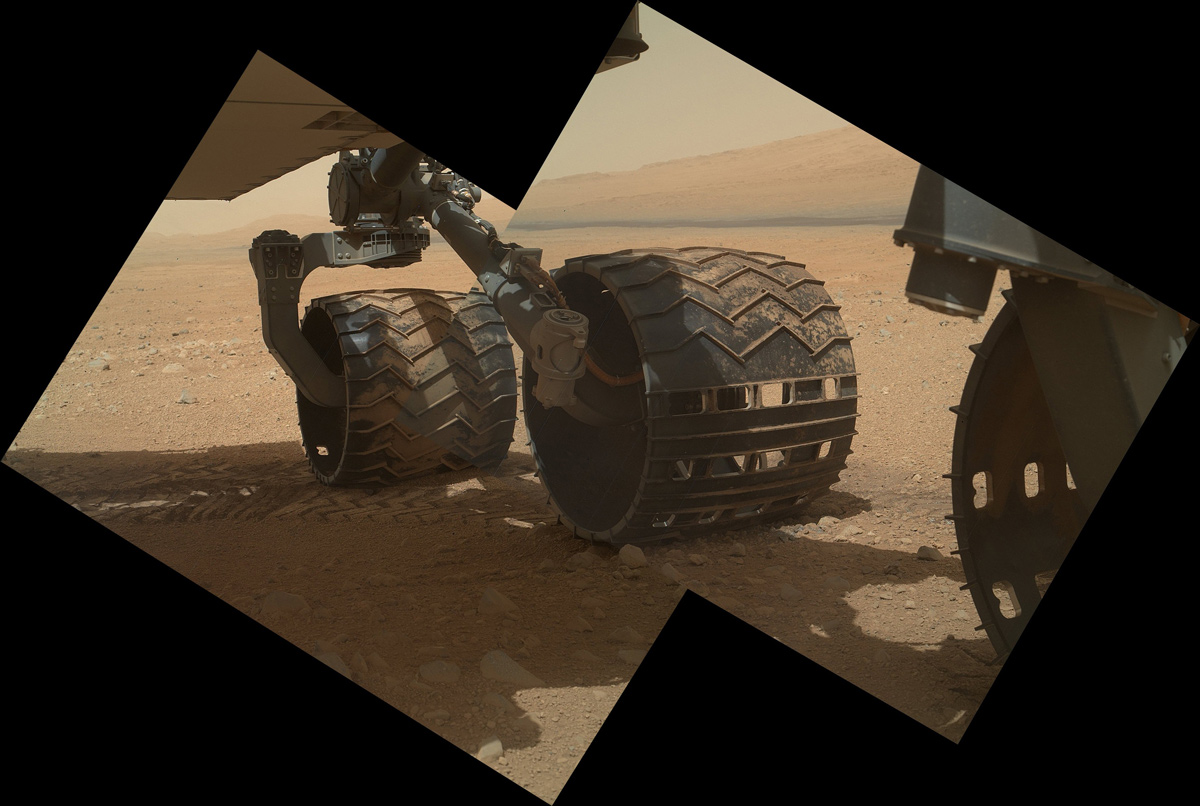
\includegraphics[width=.94\linewidth]{../../figures/mars.nasa.jpeg}
\end{center}


\begin{itemize}
\item Mass 900 kg
\item Six wheels, each with an electric motor
\item Front- and rear-wheel steering
\item Rocker-bogie suspension system
\end{itemize}
\end{column}
\end{columns}
\end{frame}

\begin{frame}[label={sec:org6f52b65}]{The problem situation}
\begin{columns}
\begin{column}{0.4\columnwidth}
\begin{center}
 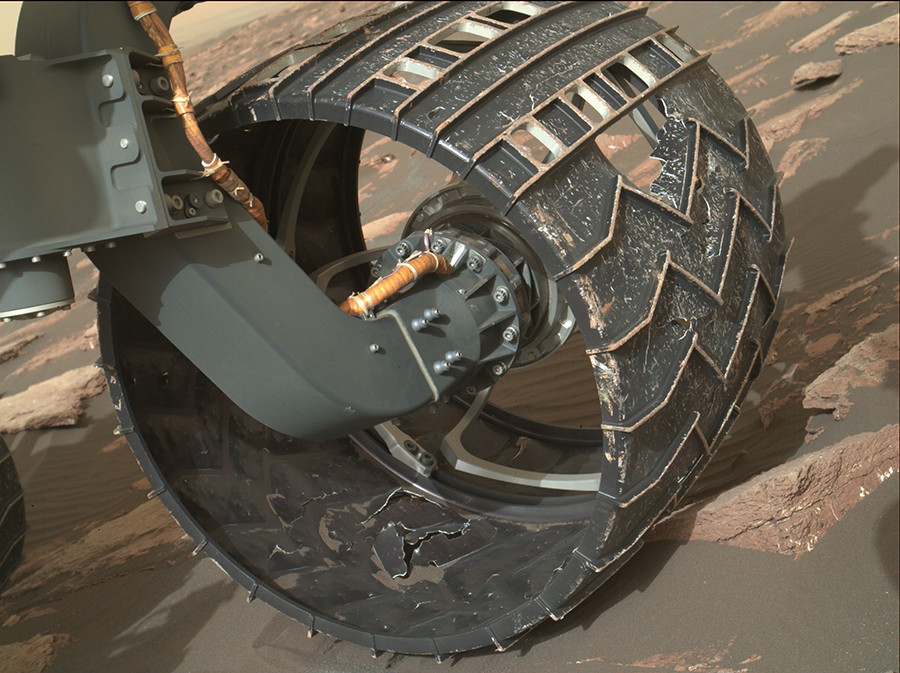
\includegraphics[width=1.0\linewidth]{../../figures/curiosity-wheel.jpg}
\end{center}
\end{column}

\begin{column}{0.6\columnwidth}
\pause

\begin{center}
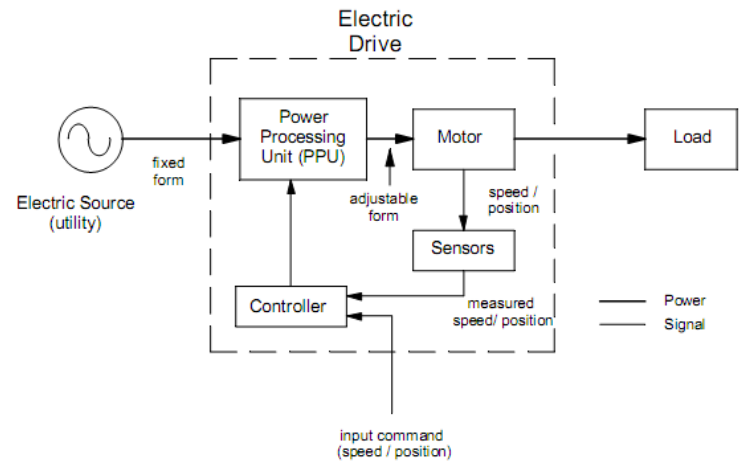
\includegraphics[width=\linewidth]{../../figures/electric-drive-block.png}
\end{center}
\end{column}
\end{columns}
\end{frame}

\section{Feedback, sensitivity and complementary sensitivity}
\label{sec:org01b3bf2}

\begin{frame}[label={sec:org9815f71}]{Block diagram algebra}
\begin{center}
  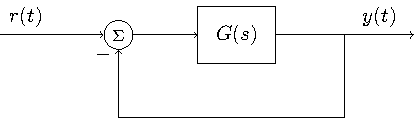
\includegraphics[width=.6\linewidth]{../../figures/block-simple-feedback}
\end{center}

Transfer function from \(r(t)\) to \(y(t)\):
\[ \frac{Y(s)}{R(s)} = \frac{G(s)}{ 1+ G(s)}\]
\end{frame}


\begin{frame}[label={sec:org02fd7d1}]{Block diagram algebra}
\alert{Activity} Pair the block-diagram with the correct closed-loop transfer function!


\begin{longtable}{cccc}
\textcolor{red}{A} & \textcolor{red}{B} & \textcolor{red}{C} & \textcolor{red}{D}\\
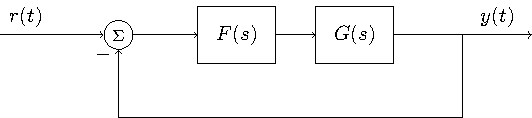
\includegraphics[width=3cm]{../../figures/block-simple-control-feedback} & 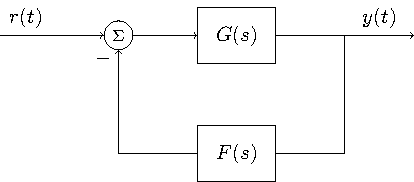
\includegraphics[width=3cm]{../../figures/block-simple-control-feedback2} & 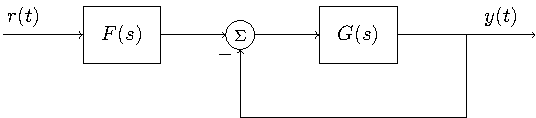
\includegraphics[width=3cm]{../../figures/block-simple-control-feedback3} & 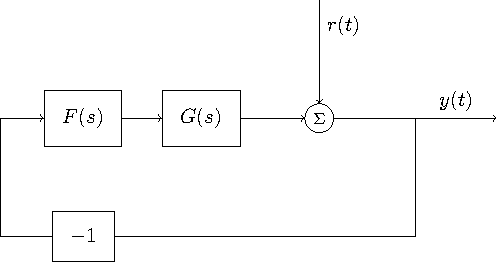
\includegraphics[width=3cm]{../../figures/block-simple-control-feedback4}\\
\end{longtable}


\begin{longtable}{cccc}
\textcolor{blue!80!black}{I} & \textcolor{blue!80!black}{II} & \textcolor{blue!80!black}{III} & \textcolor{blue!80!black}{IV}\\
\(\frac{Y(s)}{R(s)}=\frac{G(s)F(s)}{1 + G(s)}\) & \(\quad \frac{Y(s)}{R(s)}=\frac{G(s)}{1 + G(s)F(s)}\quad\) & \(\frac{Y(s)}{R(s)}=\frac{1}{1 + G(s)F(s)}\) & \(\frac{Y(s)}{R(s)}=\frac{G(s)F(s)}{1 + G(s)F(s)}\)\\
\end{longtable}
\end{frame}


\section{Control systems specifications}
\label{sec:org677b008}

\begin{frame}[label={sec:orgad4e64c}]{Performance requirements}
\begin{center}
  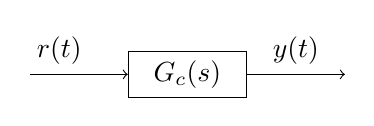
\begin{tikzpicture}[scale = 0.8, node distance=20mm, block/.style={rectangle, draw, minimum width=15mm}, sumnode/.style={circle, draw, inner sep=2pt}]

  \node[coordinate] (refinput) {};
  \node[block, right of=refinput] (motor) {$G_c(s)$};
  \node[coordinate, right of=motor, node distance=20mm] (output) {};

  \draw[->] (refinput) -- node[above, pos=0.3] (voltsignal) {$r(t)$} (motor);
  \draw[->] (motor) -- node[above, pos=0.5] (velsignal) {$y(t)$} (output);
  \end{tikzpicture}
\end{center}
\end{frame}


\begin{frame}[label={sec:org3ac524b}]{Performance requirements - time domain}
\begin{center}
  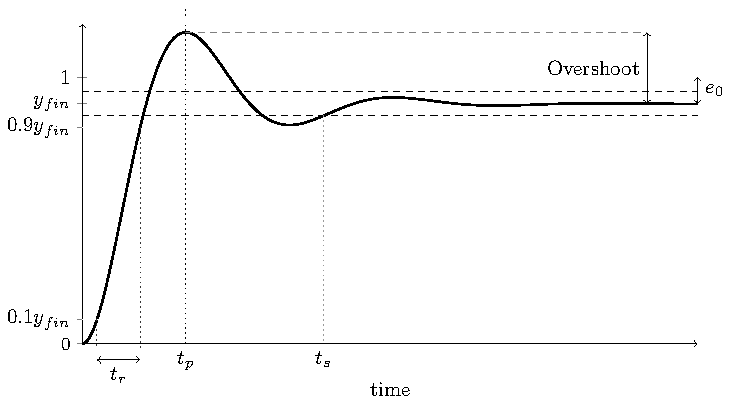
\includegraphics[width=.8\linewidth]{../../figures/step-response-specifications}
\end{center}
\end{frame}


\begin{frame}[label={sec:orge17f11d}]{Performance requirements - time domain}
\alert{Activity} Does the system satisfy the requirements?

\begin{columns}
\begin{column}{0.3\columnwidth}
\begin{center}
\begin{tabular}{ll}
Rise time & < 1.5s\\
Overshoot & < 18\%\\
\end{tabular}
\end{center}
\end{column}


\begin{column}{0.7\columnwidth}
\begin{center}
 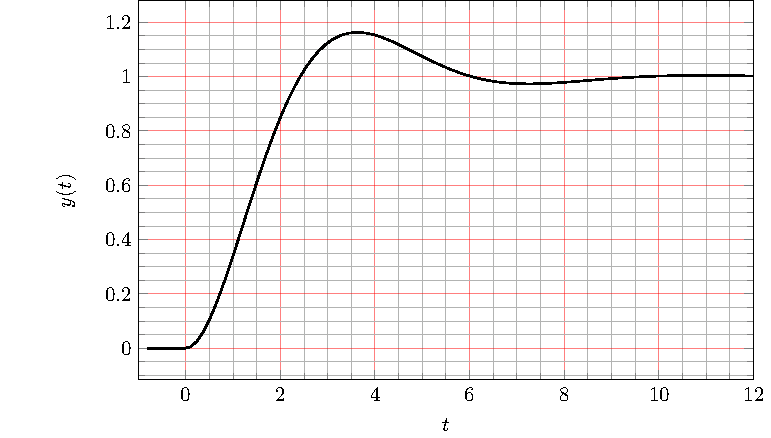
\includegraphics[width=1.0\linewidth]{../../figures/second-order-response-example}
\end{center}
\end{column}
\end{columns}
\end{frame}

\begin{frame}[label={sec:orgd004af3}]{Performance requirements - frequency domain}
\end{frame}

\begin{frame}[label={sec:org17a71c4}]{Response of LTI systems to sinusoids}
\begin{center}
  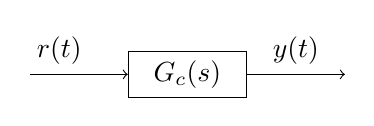
\begin{tikzpicture}[scale = 0.8, node distance=20mm, block/.style={rectangle, draw, minimum width=15mm}, sumnode/.style={circle, draw, inner sep=2pt}]

  \node[coordinate] (refinput) {};
  \node[block, right of=refinput] (motor) {$G_c(s)$};
  \node[coordinate, right of=motor, node distance=20mm] (output) {};

  \draw[->] (refinput) -- node[above, pos=0.3] (voltsignal) {$r(t)$} (motor);
  \draw[->] (motor) -- node[above, pos=0.5] (velsignal) {$y(t)$} (output);
  \end{tikzpicture}
\end{center}

Let \(r(t) = \sin\omega_1 t\). Then, after transients have died out,
\[ y(t) = |G_c(i\omega_1)| \sin \big( \omega_1 t + \arg G_c(i\omega_1)\big). \]
\end{frame}


\begin{frame}[label={sec:org3a363a2}]{The Bode diagram shows the frequency properties of a dynamical system}
\small

\[ y(t) = \underbrace{|G_c(i\omega_1)|}_{\text{amplification}} \sin \big( \omega_1 t + \underbrace{\arg G_c(i\omega_1)}_{\text{phase shift}} \big) \]


\begin{center}
  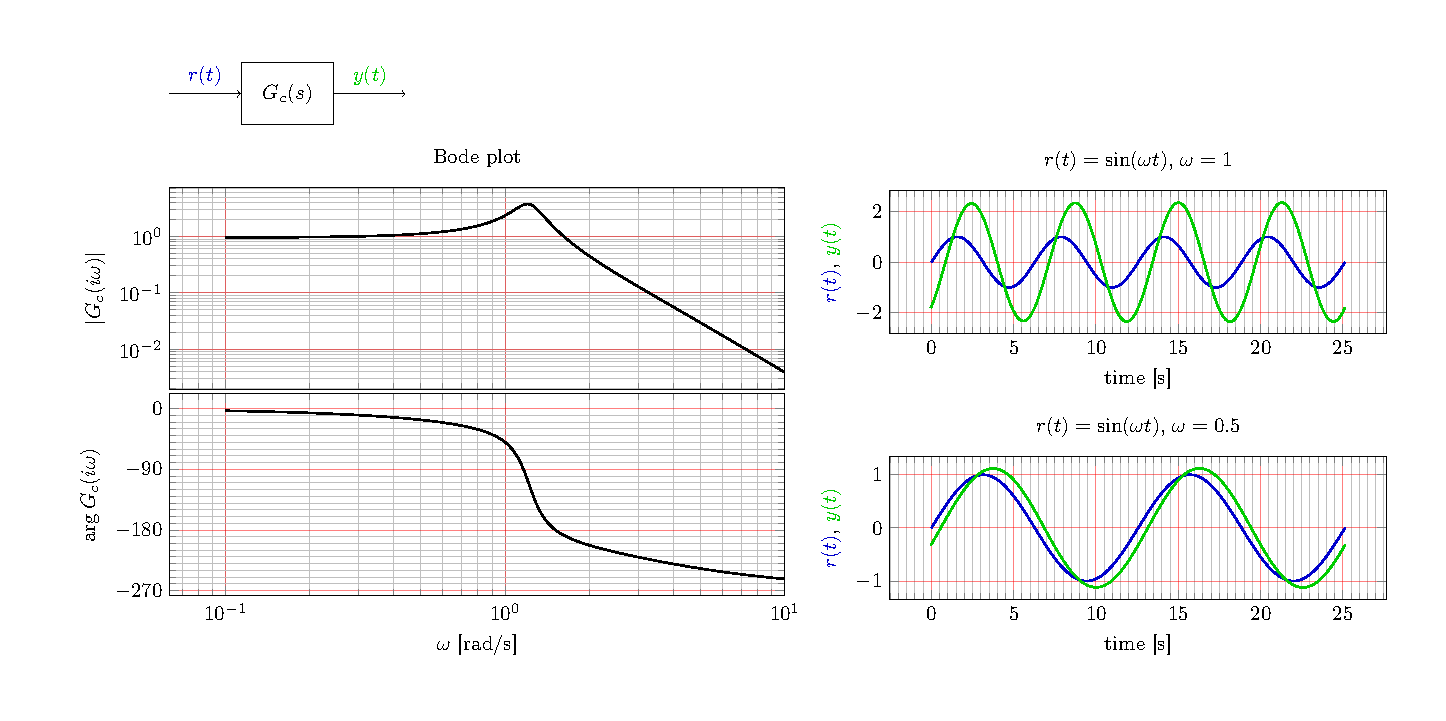
\includegraphics[width=.9\linewidth]{../../figures/bode-closed-loop-example-responses}
\end{center}
\end{frame}


\begin{frame}[label={sec:orge671087}]{Performance requirements - frequency domain}
\begin{center}
  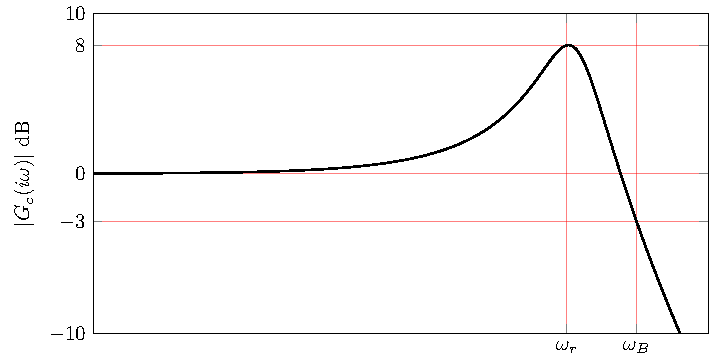
\includegraphics[width=.8\linewidth]{../../figures/spec-bode-closed-loop-new}
\end{center}
\end{frame}


\begin{frame}[label={sec:orgc811ef0}]{Performance requirements - frequency domain}
\begin{center}
  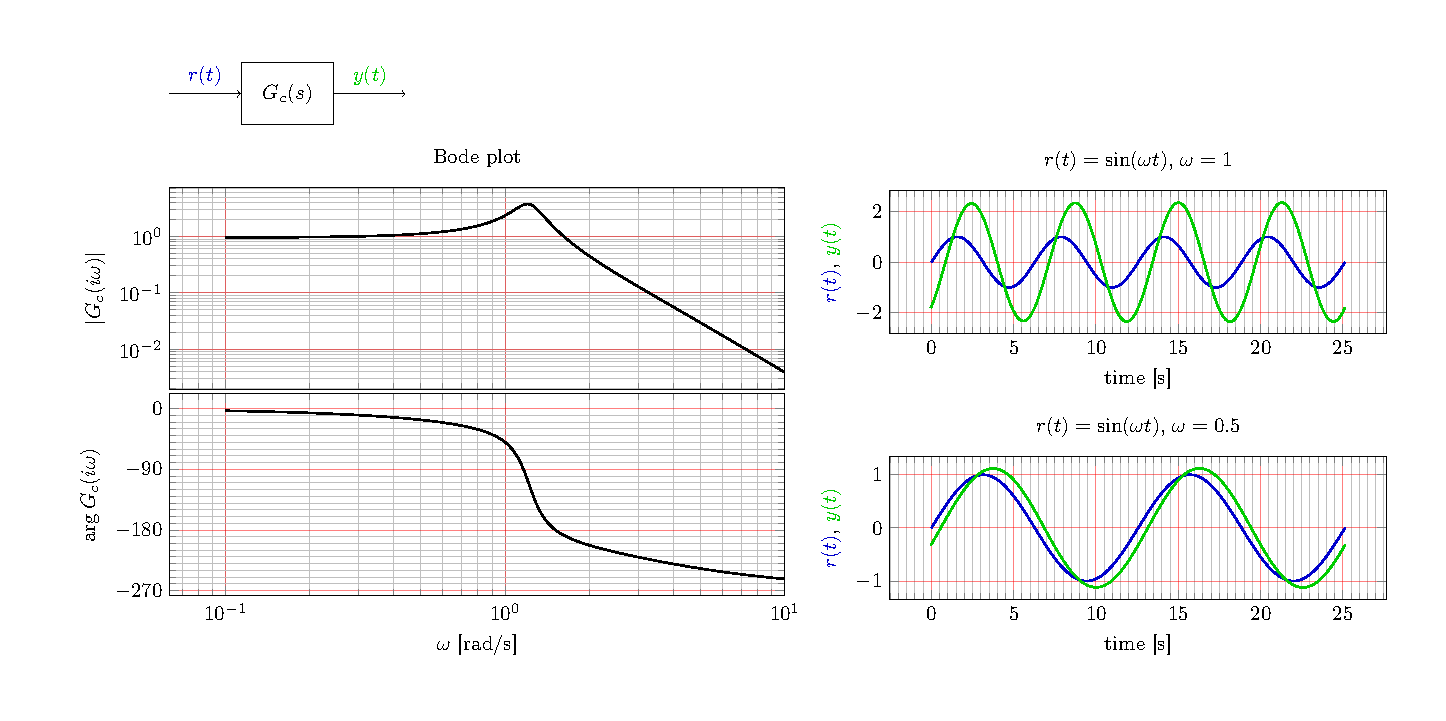
\includegraphics[width=1.0\linewidth]{../../figures/bode-closed-loop-example-responses}
\end{center}

\pause

\alert{Activity} What is the gain and phase shift at \(\omega = 2\) rad/s?
\end{frame}

\begin{frame}[label={sec:org56bb237}]{Performance requirements - frequency domain}
\begin{center}
  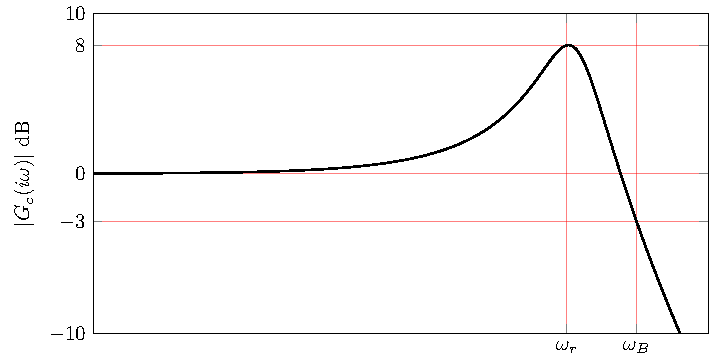
\includegraphics[width=.8\linewidth]{../../figures/spec-bode-closed-loop-new}
\end{center}
\end{frame}


\begin{frame}[label={sec:org344f278}]{Performance requirements - frequency domain}
\alert{Activity} Does the system satisfy the requirements?


\begin{columns}
\begin{column}{0.7\columnwidth}
\begin{center}
 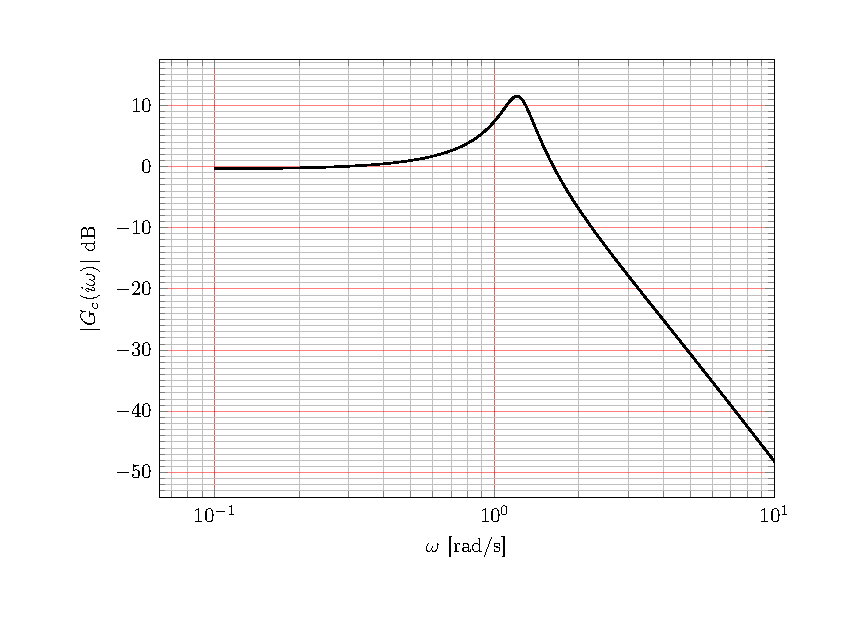
\includegraphics[width=1.0\linewidth]{../../figures/bode-closed-loop-example}
\end{center}
\end{column}
\begin{column}{0.3\columnwidth}
\begin{center}
\begin{tabular}{ll}
Bandwidth & >3 rad/s\\
Resonance peak & <9dB\\
\end{tabular}
\end{center}
\end{column}
\end{columns}
\end{frame}
\end{document}